%----------------------------------------------------
% Setup Beamer
%----------------------------------------------------
\documentclass[hyperref={colorlinks=true}]{beamer}

%----------------------------------------------------
% Packages to use
%----------------------------------------------------
\input{../packages.sty}

%----------------------------------------------------
% Setup Theme
%----------------------------------------------------
\input{../theme.sty}

%----------------------------------------------------
% Table of Contents at each section transition
%----------------------------------------------------

\AtBeginSection[]
{
   \begin{frame}
       \frametitle{Outline}
       \setcounter{tocdepth}{2}
       \tableofcontents[currentsection]
   \end{frame}
}

%----------------------------------------------------
% Colors
%----------------------------------------------------
\input{../mycolors.sty}

%----------------------------------------------------
% Style, formatting, and new commands
%----------------------------------------------------
\input{../../global.sty}
\input{../newcommands.sty}
\input{../EandMcommands.sty}

%----------------------------------------------------
% Set paths for plots and images
%----------------------------------------------------
\input{../paths.sty}


%-----------------------------------------------------------------------------------------
% Title: [Column]{Title}
%-----------------------------------------------------------------------------------------
\title[PHYS 250 (Autumn 2019) -- Lecture 5]{Ising model}

%-----------------------------------------------------------------------------------------
% SubTitle: [Column]{Subtitle}
%-----------------------------------------------------------------------------------------
\subtitle{PHYS 250 (Autumn 2019) -- Lecture 5}

%-----------------------------------------------------------------------------------------
% Author: [SubAuthor]{Author}
%-----------------------------------------------------------------------------------------
\author[D.W.~Miller]{David Miller}

%----------------------------------------------------
% Institute: [SubInst]{Institute}
%----------------------------------------------------
\institute[EFI, Chicago] 
{
  Department of Physics and the Enrico Fermi Institute\\
  University of Chicago
}

%----------------------------------------------------
% Institute: [SubInst]{Institute}
%----------------------------------------------------
\date[October 15, 2019]{October 16, 2019}

\subject{PHYS 250 Lecture}

\begin{document}

%==========================================================================================
% TITLE PAGE
%==========================================================================================

{
\begin{frame}
  \titlepage
\end{frame}
}

%==========================================================================================
\section[Plan for the Ising model]{Plan for the Ising model}
%==========================================================================================


%-----------------------------------------------------------------------------------------
\subsection[Next 3 lectures]{Next 3 lectures}
%-----------------------------------------------------------------------------------------

\begin{frame}[shrink=10]
  \frametitle{Outline of the Ising model discussion}

  This is a big topic, so I want you to have some guide for where we are going.
  
  \begin{itemize}
    \item \bluebf{Lecture 5 (Today): the model itself}
    \begin{itemize}
      \item The general concept of the Ising model: lattice of spins
      \item Basis in thermodynamics and quantum mechanics
      \item Importance of simulations methods
      \item \greenbf{Hands-on session in class: building a functional form to use for simulations}
    \end{itemize}
    \item \bluebf{Lecture 6: computational approaches}
    \begin{itemize}
      \item Continuing whatever is not covered on the model discussion from Lecture 5
      \item History of computational simulation methods: Monte Carlo
      \item The Metropolis Monte Carlo algorithm and its assumptions (deeply related to thermodynamics)
      \item \greenbf{Hands-on session in class: The Metropolis-Hastings method}
    \end{itemize}
    \item \bluebf{Lecture 7: analytical and computational evaluation}
    \begin{itemize}
      \item Analytical Ising model and the key numerical results
      \item Concept of equilibrium and how we can define it
      \item Observables in the Ising model and their calculation
      \item \greenbf{Hands-on session in class: Hands-on with Ising model simulations}
    \end{itemize}
    \item \bluebf{Hands-on lab session: Wed Oct 23rd afternoon}
    \begin{itemize}
      \item Hands-on session in CSIL 1\&2 for developing our Ising model simulation
    \end{itemize}
  \end{itemize}

\end{frame}


%==========================================================================================
\section[Ising model]{Ising model}
%==========================================================================================


%-----------------------------------------------------------------------------------------
\subsection[Statement of the problem]{Statement of the problem}
%-----------------------------------------------------------------------------------------

\begin{frame}%[shrink=10]
  \frametitle{Ising model}
  
  \setbeamercovered{transparent}
  
  In seeking to explain a particular phenomenon in physics, namely the onset of ferromagnetism, Wilhelm Lenz proposed in 1924 that his PhD student, Ernst Ising should solve a puzzling 1-dimensional model of  [\href{https://arxiv.org/abs/1706.01764}{arXiv:1706.01764}]. 
  
  \vspace{0.3cm}
  
  This model was meant to attempt to describe the interaction of \alertbf{``elementary magnetic units, which prefer alignment''}, a problem which belonged to the new and undeveloped quantum mechanics. 
  
  \vspace{0.3cm}
  
  In order to make any progress at all, Ising started in 1 dimension with the task of calculating analytically the macroscopic magnetization with the methods of statistical mechanics.
  
  \begin{figure}
    \centering
    
\includegraphics[width=\textwidth]{Ising-spins-1D.pdf}
  \end{figure}
  
  % Statement of what it is
  % How you think about it
  % Some of the physics

\end{frame}

%-----------------------------------------------------------------------------------------
\subsection[Thermodynamics and quantum mechanics]{Thermodynamics and quantum mechanics}
%-----------------------------------------------------------------------------------------

\begin{frame}%[shrink=10]
  \frametitle{Thermodynamics of the problem}
  
  \setbeamercovered{transparent}
  
  Before we go too far, let's ask the question:
  
  \begin{center}
    \alertbf{What are we really attempting to calculate?} 
  \end{center}
  
  What we want, actually, is a rather \textit{typical} thermodynamic description: 
  
  \pause
  
  \vspace{0.3cm}
  
  \begin{ucblock}{}
    \bluebf{What are relationships between macroscopic properties of the system and how will the system evolve in time towards an equilibrium state?} 
  \end{ucblock}

  For the case at hand, this becomes the specific question:
  
  \pause
  
  \vspace{0.3cm}
  
  \begin{ucblock}{}
    \bluebf{Given a randomized set of magnetic elements (think: \textit{spins!}) in $d$ dimensions, what happens to the system? Does the average spin remain random? How does the application of an external field affect its evolution? Can we calculate a specific heat for this system (the temperature change required to raise the system's energy by a given amount)?} 
  \end{ucblock}

\end{frame}

%-----------------------------------------------------------------------------------------

\begin{frame}%[shrink=10]
  \frametitle{Thermodynamics \ra statistical mechanics}
  
  \setbeamercovered{transparent}
  
  Since the microscopic properties are often (and certainly in this case) critical to understanding the answer to this question, we must -- and Ising did -- reformulate it in a statistical mechanical manner:
  
  \pause
  
  \vspace{0.1cm}
  
  \begin{ucblock}{}
    \bluebf{What are the microscopic properties of a system that govern how that system will evolve in time, and what is the process by which is will undergo that evolution?} 
  \end{ucblock}
  
  \vspace{0.1cm}
  
  \pause
  
  To answer this question, we have to understand several things:
  
  \begin{itemize}[<+->]
    \item \textit{How do we even talk about the microscopic state of a system like this?}
    \item \textit{What properties matter?}
    \item \textit{What causes the system to evolve?}
    \item \textit{What is the likelihood that it evolves in a particular direction?}
  \end{itemize}

  These are seemingly simply questions that belie a deep set of physical principles and, since we're here, computational techniques.

\end{frame}

%-----------------------------------------------------------------------------------------

\begin{frame}%[shrink=10]
  \frametitle{What properties and states are we interested in? (Energy!)}

  \setbeamercovered{transparent}

  As you've probably seen in so many of your courses by now, the energy of the system is a critical piece of understanding its evolution.
  
  \vspace{0.3cm}
  
  In the case of \bluebf{thermodynamics} perhaps you have heard that the \alertbf{temperature} of the system is a property that we use to describe or \textit{map} on to the state of the system, and hence its energy.

  \begin{figure}
    \centering
    \frame{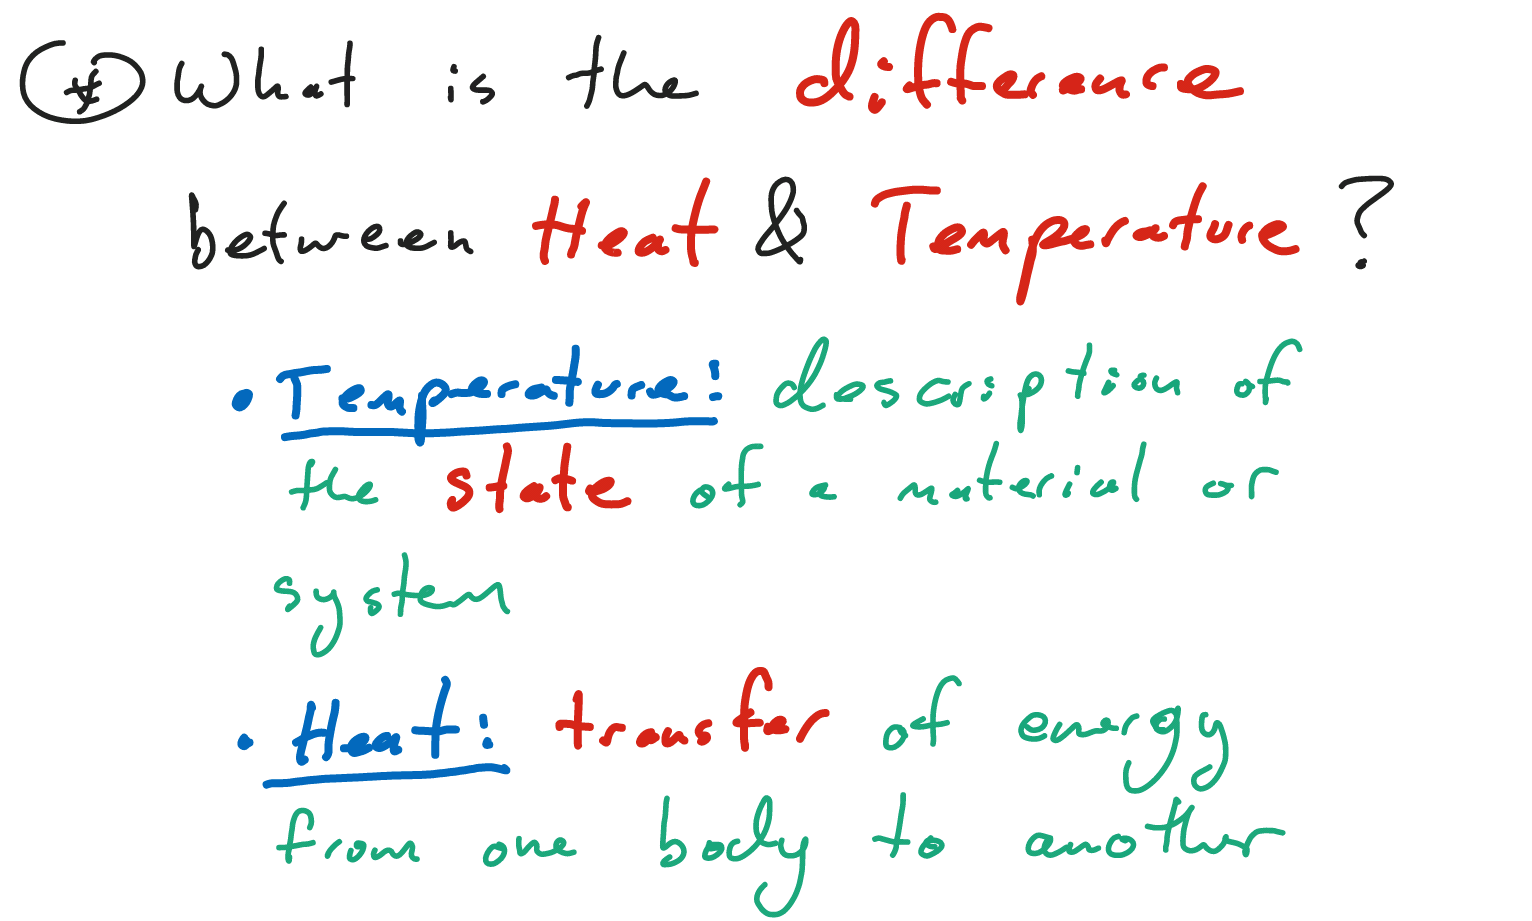
\includegraphics[width=0.65\columnwidth]{Temperature.png}}
    \caption{From my PHYS 133 notes}
  \end{figure}

\end{frame}

%-----------------------------------------------------------------------------------------

\begin{frame}%[shrink=10]
  \frametitle{What drives the evolution of the system?}
  
  \setbeamercovered{transparent}

  What causes a system to \bluebf{evolve} is the tendency towards an equilibrium state. This is effectively embodied in the second law of thermodynamics which states:
  
  \pause
  
  \begin{ucblock}{Second law of thermodynamics}
    The total entropy of an isolated system can never decrease over time. In all spontaneous processes, the total entropy increases and the process is irreversible. 
  \end{ucblock}
  
  \pause
  
  Ultimately, this means that when a system starts from an equilibrium state, is then \textit{perturbed} by a thermodynamic operation (e.g. bringing two components of the system of different temperatures into contact), it will spontaneously (given some relaxtion time) reach its own new state of internal thermodynamic equilibrium.
  
  \vspace{0.3cm}
  
  Statistical mechanics essentially \textit{explains} this law via an understanding of the micro states of the system.

\end{frame}


%-----------------------------------------------------------------------------------------

\begin{frame}%[shrink=10]
  \frametitle{Probability distribution for a particular set of states}

  Part of our task is therefore to count the various energy configurations based on the possible \textit{microscopic states} (or \textit{microstates}) of the system in order to determine the \alertbf{partition function}, which tells us how the states are distributed given their energies:
  
  \pause
  
  \begin{equation}
    Z = \sum_i e^{-\beta \Ham_i}
  \end{equation}

  where $\beta$ is the inverse ``temperature'' of the system, $\beta = (\kB T)^{-1}$ and \Ham is the Hamiltonian of the system, the expectation value of which is the energy, $E_i$, of that microstate, $i$. \pause The configuration probability of an ensemble of microstates 
  
  \begin{equation}
    P = \frac{e^{-\beta \Ham_i}}{Z}
  \end{equation}

  \pause

  Since the total probability to find the system in some microstate must be equal to 1, the partition function serves as the normalization constant. In \textit{classical} systems, we'd merely obtain the expectation value by taking an integral over the appropriate volume in order to turn the exponential into a sum over energy states.

\end{frame}
%-----------------------------------------------------------------------------------------

\begin{frame}%[shrink=10]
  \frametitle{Boltzmann distribution and the ``canonical ensemble''}
  
  \begin{columns}
  
  \column{0.5\textwidth}
  
  You may have noticed the Boltzmann factor on the previous slide:
  
  \begin{equation}
    e^{-\beta E_i}
  \end{equation} 

  \pause

  This comes from the basic idea that \bluebf{the number of states decreases exponentially for high energies when the temperature is fixed}. This again is a very basic idea, but is crucial to understand the physics. An ensemble of micro states (e.g. particles) that follow this distribution is referred to as the \bluebf{canonical ensemble}. 
  
  \column{0.45\textwidth}
  
    \pause
  
    \begin{figure}
      \centering
      \frame{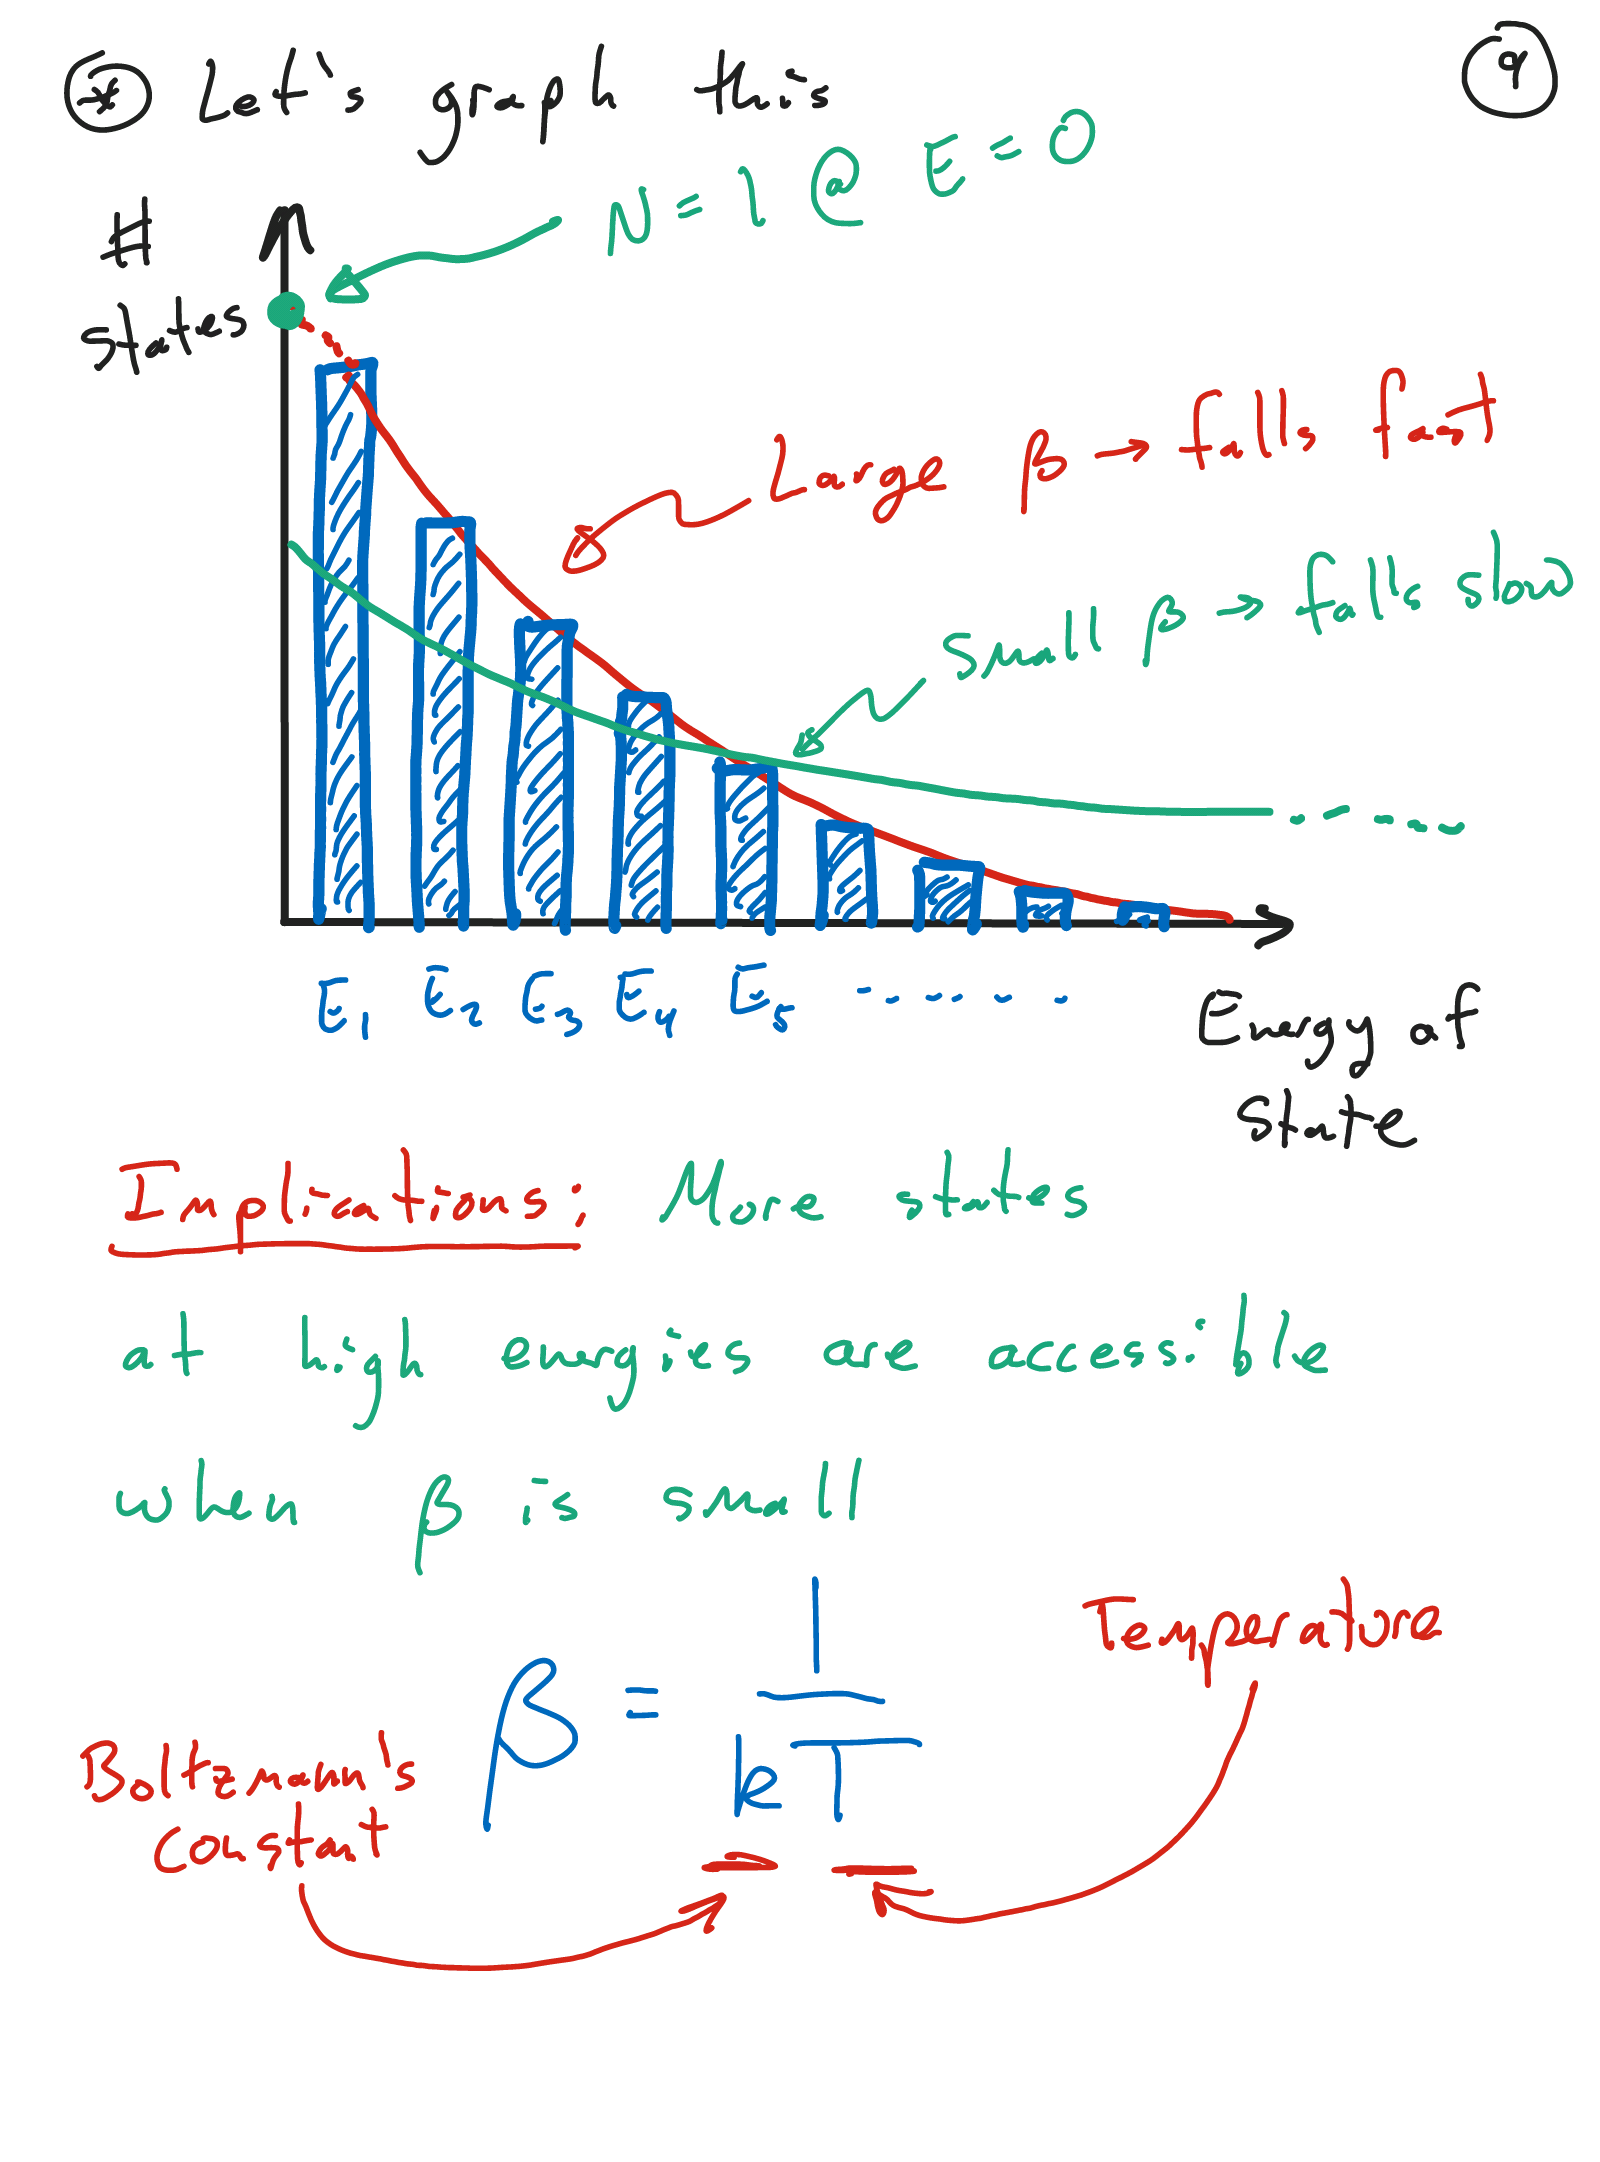
\includegraphics[width=\columnwidth]{Boltzmann.png}}
    \end{figure}
  
  \end{columns}

  \pause 
  
  \centering \alertbf{Hand's on with the \texttt{MaxwellBoltzmann.ipynb} notebook!}

\end{frame}

%-----------------------------------------------------------------------------------------

\begin{frame}%[shrink=10]
  \frametitle{Quantum mechanics of the Ising model}

  \begin{columns}
  
  \column{0.5\textwidth}
  
  The Hamiltonian for a system of $N$ spins $s_i$ in free space, which may take on values of $s_i = \pm1$ is given by the interaction of the spins
  %
  \begin{equation}
    \Ham = -J \sum_{\mean{ij}}^N s_i s_{j} , \label{eq:ising-free}
  \end{equation} 
  %
  where the sum \mean{ij} is over all pairs of nearest-neighbor sites, $J$ is the \alertbf{coupling} between these neighboring sites. (For example, there are four neighbors per site on the square lattice.)
  
  \vspace{-0.5cm}
  
    \begin{figure}
      \centering
      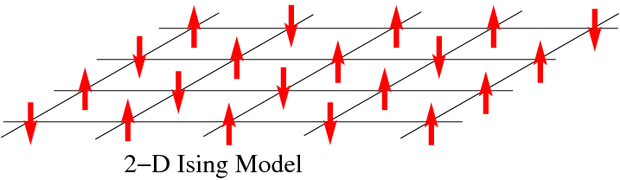
\includegraphics[width=0.8\columnwidth]{Ising-spins-2D.png}
    \end{figure}
    
  \column{0.45\textwidth}
  
    \begin{figure}
      \centering
      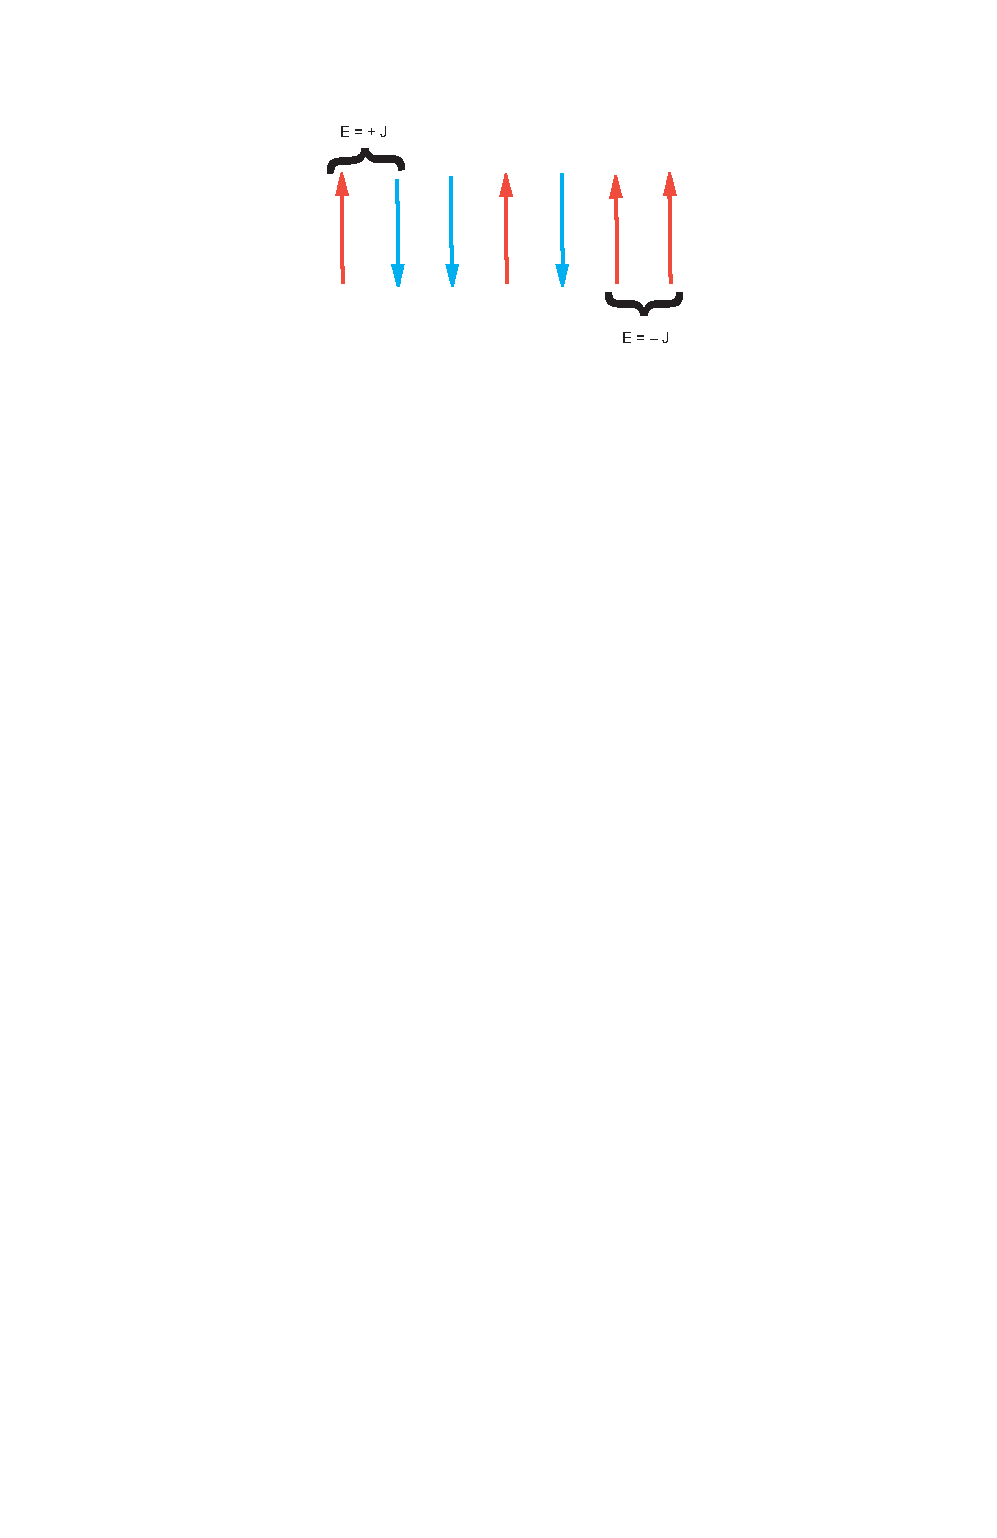
\includegraphics[width=\columnwidth]{Ising-spins-1D-interaction.pdf}\\
      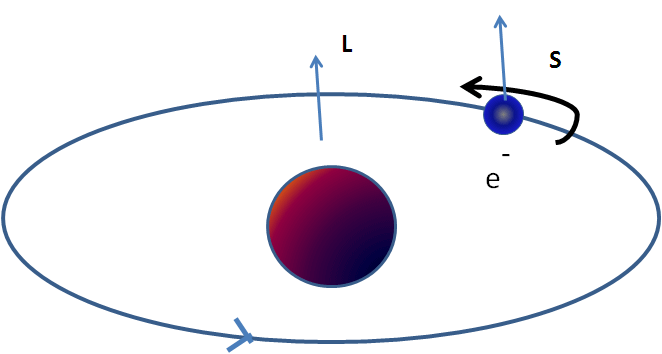
\includegraphics[width=\columnwidth]{SpinOrbitMoment.png}
    \end{figure}
  
  \end{columns}

  

\end{frame}

%-----------------------------------------------------------------------------------------

\begin{frame}%[shrink=10]
  \frametitle{Magnetism and spins (I)}

  As we've discussed in E\&M, magnetism is caused by charged particles \bluebf{``spinning''} in closed orbits or about their axes
  %
  \begin{itemize}
    \item For elementary particles, of course, we mean ``spinning'' in the quantum mechanical sense, not the rotational Newtonian sense
  \end{itemize}
  %
  So atoms may have \bluebf{both an $L$ (orbit) and an $S$ (spin) contribution} (capital letters for ``operators'' for those of you in the know) to the magnetic properties. For the Ising model, we're concerned with just a single contribution which we will refer to as $s$ as on the previous slide.
  
  \vspace{0.3cm}
  
  In addition to the contribution to the Hamiltonian (and thus the energy) from the spin-spin interactions, there is the possibility that we apply an external magnetic field, $H$:
  %
  \begin{equation}
    \Ham = -J \sum_{\mean{ij}}^N s_i s_{j} - H \sum_i s_i , \label{eq:ising-field}
  \end{equation} 

  Note that the ``magnetization'' is given by $M=\sum_i s_i$.

\end{frame}



%-----------------------------------------------------------------------------------------

\begin{frame}%[shrink=10]
  \frametitle{Magnetism and spins (II)}

  Let's discuss our Hamiltonian
  %
  \begin{equation}
    \Ham = -J \sum_{\mean{ij}}^N s_i s_{j} - H \sum_i s_i , \label{eq:ising-field}
  \end{equation} 
  %
  \begin{itemize}
    \item \bluebf{If $J > 0$ : ferromagnetic}
    \begin{itemize}
      \item Energy is minimized if the spins point in the same direction
    \end{itemize}
    \item \bluebf{If $J < 0$ : antiferromagnetic}
    \begin{itemize}
      \item Energy is minimized if spins locally point in the opposite direction
    \end{itemize}
  \end{itemize}
  
  \begin{ucblock}{Important observations which we will study}
    \begin{itemize}
      \item At low temperatures, the \bluebf{spins will organize themselves} to either mostly point up or mostly point down, forming a ferromagnetic phase.
      \item The spins will tend to align (in a 2D square lattice) in a \bluebf{checkerboard antiferromagnetic phase} at low temperatures. 
      \item At high temperatures, independent of the sign of $J$, we expect entropy to dominate; the spins will fluctuate wildly in a \bluebf{paramagnetic phase} and the magnetization per spin $m(T ) = M (T )/N$ is zero 
    \end{itemize}
  \end{ucblock}
    
\end{frame}

%-----------------------------------------------------------------------------------------

\begin{frame}%[shrink=10]
  \frametitle{Emergent properties of the Ising model}
  
    \begin{figure}
      \centering
      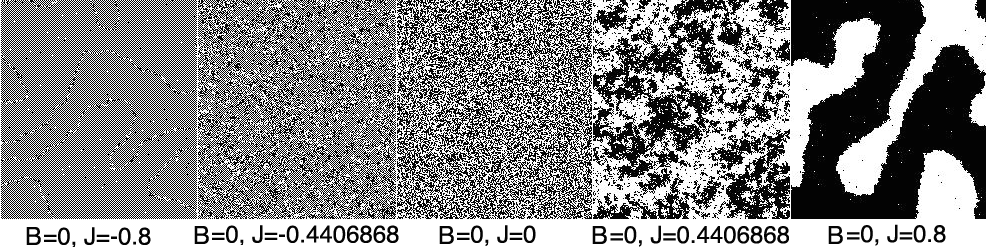
\includegraphics[width=\columnwidth]{IsingDomains.png}
    \end{figure}
  
  Amazing features result from the \bluebf{ensemble behavior} of the lattice sites of a 2D Ising model. Phase transitions, criticality, and other phenomena are all part of what we will study computationally with this model. 

  \begin{figure}
      \centering
      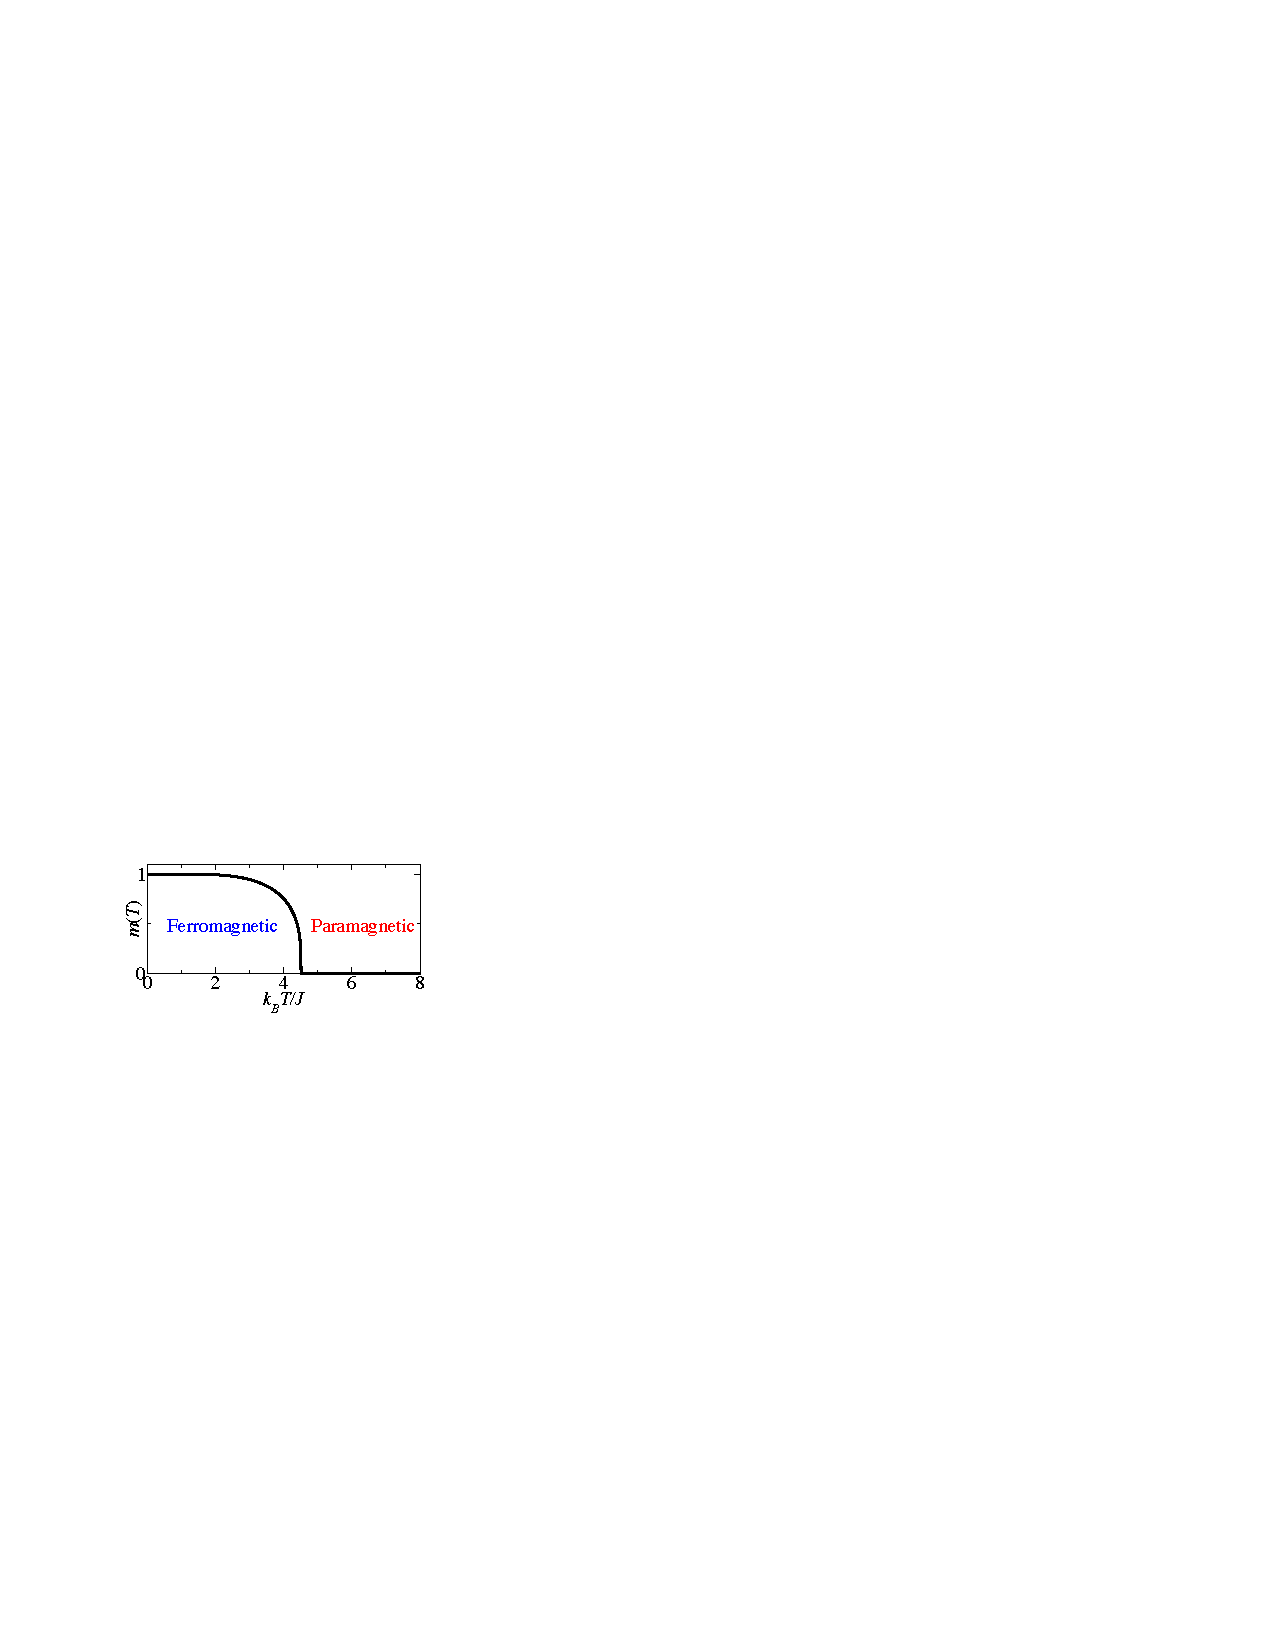
\includegraphics[width=0.5\columnwidth]{MagnetizationPerSpin.pdf}
  \end{figure}
  
\end{frame}


%-----------------------------------------------------------------------------------------

\begin{frame}%[shrink=10]
  \frametitle{A few quantum mechanics notes}
  
  The Ising model parameters are rescaled from the microscopic ones. The Ising spin $s_i = \pm1$ represents twice the $z$-component of a spin-1/2 atom in a crystal, $\sigma_i^z = s_i/2$. 
  
  \vspace{0.5cm}
  
  The Ising interactions between spins, $J s_i s_j = 4 J \sigma_i^z \sigma_j^z$, is thus shifted by a factor of four from the $z-z$ coupling between spins. 
  
  \vspace{0.5cm}
  
  The coupling of the spin to the external magnetic field is microscopically $g \mu_B H \cdot \sigma_i^z$, where $g$ is the gyromagnetic ratio for the spin (close to two for the electron) and $\mu_B = \frac{e \hbar}{2 m_e}$ is the Bohr magneton. 
  
  \vspace{0.5cm}
  
  \bluebf{Hence, for those of you who've taken quantum mechanics, the Ising external field is rescaled from the physical one by $g \mu_B / 2$. }

\end{frame}



%-----------------------------------------------------------------------------------------
\subsection[Practical implications and relationships]{Practical implications and relationships}
%-----------------------------------------------------------------------------------------

\begin{frame}%[shrink=10]
  \frametitle{Broader context for the Ising model}
  
  Lattice models are a big industry within statistical mechanics. Many systems and their computational evaluation and study take place on a lattice:
  
  \begin{itemize}
    \item \bluebf{Critical phenomena and phase transitions}
    \item \bluebf{lattice QCD and quantum field theories}
    \item \bluebf{quantum magnetism and models for high-temperature superconductors}
    \item \bluebf{phase diagrams for alloys}
    \item \bluebf{the behavior of systems with dirt or disorder}
    \item \bluebf{non-equilibrium systems exhibiting avalanches and crackling noise}
  \end{itemize}
  
  And many more!
  
  \center \textit{(now do you see why I spent time showing you \texttt{np.mgrid}?!)}
  
\end{frame}

%-----------------------------------------------------------------------------------------
\subsection[Complications and numerical and computational obstacles]{Complications and numerical and computational obstacles}
%-----------------------------------------------------------------------------------------

%-----------------------------------------------------------------------------------------

\begin{frame}%[shrink=10]
  \frametitle{Computational complexity and simulation}
  
  The 1D model was solved analytically in 1924. 
  
  \vspace{0.3cm}
  
  The 2D model was not solved analytically until Lars Onsager did it in 1944. 
  \begin{itemize}
    \item Onsager solved is using the \bluebf{ transfer-matrix method}, where you essentially break up the partition function, $Z$ into many pieces and decompose the interactions in a matrix formulation and then do an eigenvector decomposition and solve it that way. 
  \end{itemize}
  
  \vspace{0.3cm}
  
  However, this only really works for a small system. If there are many states (i.e. many sites) it can easily become analytically intractable even if solvable in principle.
  
  \vspace{0.3cm}
  
  \begin{ucblock}{}
     \textbf{Instead, we will approach this using our Monte Carlo based approach!}
  \end{ucblock}
   
\end{frame}

%%==========================================================================================
%\section[Simulation methods]{Simulation methods}
%%==========================================================================================
%
%%-----------------------------------------------------------------------------------------
%\subsection[Monte Carlo Methods]{Monte Carlo Methods}
%%-----------------------------------------------------------------------------------------
%
%
%\begin{frame}%[shrink=10]
%  \frametitle{Heat-bath Monte Carlo}
%  
%  One of the simplest approaches would be ``brute force:''
%  
%  \begin{enumerate}
%    \item Pick a site $i = (x,y)$ at random. 
%    \item Check how many neighbor spins are pointing up:
%    \begin{equation}
%      m_i = \sum _{j:\mean{ij}} s_j = \begin{cases}
%               +4  (\mathrm{4\, neighbors\, up}),\\
%               +2  (\mathrm{3\, neighbors\, up}),\\
%                0  (\mathrm{2\, neighbors\, up}),\\
%               -2 (\mathrm{1\, neighbors\, up}),\\
%               -4 (\mathrm{0\, neighbors\, up}),\\
%            \end{cases}
%    \end{equation}
%    \item Calculate $E_{+} = - J m_i - H$ and $E_{-} = +J m_i + H$, the energy for spin $i$ to be $+1$ or $-1$ given its current environment.
%    \item Set spin $i$ up with probability $P_{\mathrm{up}} = e^{-\beta E_{+}} / (e^{-\beta E_{+}} + e^{-\beta E_{-}})$ and down with probability $P_{\mathrm{down}} = e^{-\beta E_{-}} / (e^{-\beta E_{+}} + e^{-\beta E_{-}})$.
%    \item Repeat.
%  \end{enumerate}
%
%\end{frame}
%%-----------------------------------------------------------------------------------------
%%\subsection[Accept-reject algorithms]{Accept-reject algorithms}
%%-----------------------------------------------------------------------------------------
%
%%-----------------------------------------------------------------------------------------
%\subsection[Metropolis-Hastings algorithm]{Metropolis-Hastings algorithm}
%%-----------------------------------------------------------------------------------------
%
%%-----------------------------------------------------------------------------------------
%
%
%\begin{frame}%[shrink=10]
%  \frametitle{Metropolis Monte Carlo (II)}
%  
%  The heat bath approach tries to essentially set the whole lattice state by iterating over the whole grid one site at a time. However, we can use the magic of the MCMC approach to try to do this much more efficiently. Instead, let's represent the \alertbf{entire lattice} at once and ask:
%  
%  \vspace{0.3cm}
%  
%  \begin{ucblock}{}
%    \alertbf{What is the probability that the whole system transitions from one state (i.e. set of spins) to another?}
%  \end{ucblock}
%  
%  \vspace{0.3cm}
%  
%  An $N$-state Ising model has $2^N$ states $\mathbb{S} = \{s_i\}$. A Markov chain for the Ising model has a transition rule, which at each step shifts the current state $\mathbb{S}$ to a state $\mathbb{S}^{\prime}$ with probability $P_{\mathbb{S}\Leftarrow\mathbb{S}^{\prime}}$.
%  
%  \vspace{0.3cm}
%  
%  For the heat-bath algorithm, $P_{\mathbb{S}\Leftarrow\mathbb{S}^{\prime}}$ is equal to zero unless $\mathbb{S}^{\prime}$ and $\mathbb{S}$ the same except for at most one spin flip.
%
%\end{frame}
%
%%-----------------------------------------------------------------------------------------
%
%
%\begin{frame}%[shrink=10]
%  \frametitle{Metropolis Monte Carlo (I)}
%  
%  ``Pseudocode'' for the Metropolis algorithm:
%  
%  \begin{enumerate}
%    \item Choose initial configuration
%    \item For all spins:
%    \begin{enumerate}
%      \item Trial flip ($+1 \ra -1$ or vice versa)
%      \item Compute change in energy
%      \item If $\delta = e^{\Delta E/\kB T} > r$ (where $r$ is a uniform deviate) flip the spin 
%    \end{enumerate}
%  \end{enumerate}
%  
%  But we can do even better! Next time!
%  
%\end{frame}
%
%




%%==========================================================================================
%\section[Conclusions]{Conclusions}
%==========================================================================================
%
%\begin{frame}%[shrink=1]
%  \frametitle{Conclusions}
%
%  \begin{itemize}
%    \item Something
%  \end{itemize}
%  
%\end{frame}

%==========================================================================================
%==========================================================================================
\end{document}
